% Source: http://tex.stackexchange.com/a/150903/23931
\documentclass[a4paper, 11pt]{article}
\topmargin-2.0cm
\usepackage{fancyhdr}
\usepackage{amsfonts}
\usepackage{pagecounting}
\usepackage{caption}
\usepackage{subcaption}
\usepackage[shortlabels]{enumitem}
\usepackage{graphicx}
\usepackage{adjustbox}
\usepackage{xcolor}
\usepackage{times}
\usepackage{mathrsfs}
\usepackage{dirtytalk}
\usepackage{amsmath}
\usepackage{semantic}
\usepackage{proof}
\usepackage{mathpartir}
\usepackage{gb4e}
\usepackage{natbib}
\usepackage{authblk}
\usepackage{booktabs}
\usepackage{array}

\setcounter{table}{0}
\renewcommand{\thetable}{\Alph{table}}
\newcolumntype{L}{>{\arraybackslash}m{13cm}}
% \usepackage{emoji}
\noautomath

\definecolor{darkblue}{rgb}{0, 0, 0.5}
\definecolor{blu}{HTML}{005082}

\newcommand{\blank}{$\rule{0.6cm}{0.15mm}$}

\usepackage[colorlinks = true,
           linkcolor = darkblue,
           urlcolor  = darkblue,
           citecolor = darkblue,
           anchorcolor = darkblue]{hyperref}

           \usepackage{cleveref}

\usepackage[margin=1in]{geometry}
% \advance\oddsidemargin-0.95in
% \advance\evensidemargin-1.5cm
% \textheight9.2in
% \textheight10.3in
% \textwidth6.75in
% \newcommand\bb[1]{\mbox{\em #1}}
% \def\baselinestretch{1.05}
%\pagestyle{empty}

\newcommand{\hsp}{\hspace*{\parindent}}
\definecolor{gray}{rgb}{0.4,0.4,0.4}
%\definecolor{gray}{rgb}{1.0,1.0,1.0}

\newcommand{\todo}[1]{\textcolor{green}{#1}}
\renewcommand\cite{\citep}	% to get "(Author Year)" with natbib    
\newcommand\shortcite{\citeyearpar}% to get "(Year)" with natbib    
\newcommand\newcite{\citet}	% to get "Author (Year)" with natbib  

\title{\textbf{Supplementary Materials: Do language models learn typicality judgments from text?}}
% \author{
%     Kanishka Misra\\
%     Purdue University, West Lafayette, IN, USA\\
%     \texttt{kmisra@purdue.edu}
% }
\author[1]{Kanishka Misra}
\author[2]{Allyson Ettinger}
\author[1]{Julia Taylor Rayz}
\affil[1]{Purdue University, West Lafayette, IN, USA}
\affil[2]{University of Chicago, Chicago, IL, USA}
\affil[1]{\texttt{\{kmisra, jtaylor1\}@purdue.edu}}
\affil[2]{\texttt{aettinger@uchicago.edu}}
\date{
}


\begin{document}
\maketitle
\thispagestyle{fancy}
%\pagenumbering{gobble}
%\fancyhead[location]{text} 
% Leave Left and Right Header empty.
\lhead{}
\rhead{}
%\rhead{\thepage}
\renewcommand{\headrulewidth}{0pt} 
\renewcommand{\footrulewidth}{0pt} 

%\pagestyle{myheadings}

\pagestyle{fancy}
\lhead{\textcolor{gray}{\it Kanishka Misra}}
% \rhead{\textcolor{gray}{\thepage/\totalpages{}}}
\rhead{\textcolor{gray}{\it Supplementary Materials: Misra, Ettinger, and Rayz (2021)}}

\section{Code}
The code and data materials used to reproduce the analyses reported in the paper can be found in the following link: \url{https://github.com/kanishkamisra/typicalityprobing}. The code is predominantly written using the \texttt{minicons}\footnote{\url{https://github.com/kanishkamisra/minicons}} library.

\section{Models Studied}

\section{Stimuli Generation}
In this section we describe in detail the language stimuli used in our two experiments. 
These stimuli have been summarized in Table 2 in the original paper.

\subsection{Categories and Exemplars from \citet{rosch1975cognitive}}
We collect our categories and their items/exemplars from the typicality ratings collected by \citet{rosch1975cognitive}.
In total, we have 565 items spanning across 10 different categories.
\Cref{tab:exemplar} shows the most and least typical items for each of the 10 categories.
We use this dataset as the ground truth resource to construct our stimuli for both our experiments.

\def\arraystretch{1.5}
\begin{table}[!t]
    \centering
    \caption{Categories and Exemplars extracted from \citet{rosch1975cognitive}. The `Exemplar' column shows 10 most and 10 least typical items for their corresponding category, as rated by native English speakers.}
    \label{tab:exemplar}
    \begin{tabular}{|c|L|}
    \hline
    \textbf{Category} &
      \multicolumn{1}{c|}{\textbf{Exemplar}} \\ \hline
    toy &
      \textit{doll, top, jack-in-the-box, toy soldier, yo-yo, block, marbles, rattle, stuffed animal, water pistol, ..., bow and arrow, rope, dishes, cards, mitt, horse, gun, animals, tennis racket, books} \\ \hline
    bird &
      \textit{robin, sparrow, bluejay, bluebird, canary, blackbird, dove, lark, swallow, parakeet, ..., duck, peacock, egret, chicken, turkey, ostrich, titmouse, emu, penguin, bat} \\ \hline
    sport &
      \textit{football, baseball, basketball, tennis, softball, canoeing, handball, rugby, hockey, ice hockey, ..., pool, billiards, hunting, jump rope, camping, chess, dancing, checkers, cards, sunbathing} \\ \hline
    vegetable &
      \textit{pea, carrot, green bean, string bean, spinach, broccoli, asparagus, corn, cauliflower, brussels sprouts, ..., escarole, sauerkraut, pickle, baked bean, pumpkin, seaweed, garlic, dandelion, peanut, rice} \\ \hline
    tool &
      \textit{saw, hammer, ruler, screwdriver, drill, nail, tape measure, sawhorse, sandpaper, sander, ..., plaster, wheelbarrow, axe, slide rule, cement, anvil, hatchet, rag, scissor, crane} \\ \hline
    fruit &
      \textit{orange, apple, banana, peach, pear, apricot, tangerine, plum, grape, nectarine, ..., pawpaw, coconut, avocado, pumpkin, tomato, nut, gourd, olive, pickle, squash} \\ \hline
    clothing &
      \textit{pant, shirt, dress, skirt, blouse, suit, slack, jacket, coat, sweater, ..., handkerchief, purse, hairband, ring, earring, watch, cuff link, necklace, bracelet, cane} \\ \hline
    vehicle &
      \textit{automobile, station wagon, truck, car, bus, taxi, jeep, ambulance, motorcycle, streetcar, ..., rocket, blimp, skate, camel, feet, ski, skateboard, wheelbarrow, surfboard, elevator} \\ \hline
    furniture &
      \textit{chair, sofa, couch, table, easy chair, dresser, rocking chair, coffee table, rocker, love seat, ..., counter, clock, drape, refrigerator, picture, closet, vase, ashtray, fan, telephone} \\ \hline
    weapon &
      \textit{gun, pistol, revolver, machine gun, rifle, switchblade, knife, dagger, shotgun, sword, ..., word, hand, pipe, rope, airplane, foot, car, screwdriver, glass, shoe} \\ \hline
    \end{tabular}
    \end{table}
    
\subsection{Taxonomic Sentence Verification}
\paragraph{Recap} Our taxonomic sentence verification experiments test whether the model's attribution of hypernyms to noun concepts---by means of word prediction in context---reflects the graded structure of concepts as observed in humans.
To this end, we compare the models' log probability of assigning an item (\textit{robin}) its superordinate category (\textit{bird}) to its typicality rating for the category as produced by humans in the original study.

\paragraph{Construction} To construct the stimuli for this experiment, we create simple English templates:
\begin{quotation}
    \centering
    \texttt{\{A/An/$\phi$\} [ITEM] \{is/are\} \{a/an/$\phi$\} [CATEGORY]}.
\end{quotation}
where \texttt{\{.\}} denotes an optional word---with options separated by a `/'---and $\phi$ is a null character.
Check out \url{https://github.com/kanishkamisra/typicalityprobing/python/} for detailed stimuli samples.

\subsection{Category-based Induction}
\paragraph{Recap} Our category-based induction experiments test whether models reflect typicality effects when making inductive generalizations. That is, are models more likely to generate \textit{``All \textbf{\textcolor{blu}{birds}} can dax''} when given \textit{``\textbf{\textcolor{blu}{Robins}} can dax,''} as opposed to \textit{``\textbf{\textcolor{blu}{Penguins}} can dax''}?

\paragraph{Construction} Following \citet{osherson1990category}, we use \textit{blank} properties in this experiment -- i.e., properties that we estimate to be vaguely unfamiliar to language models (analogous to what \citeauthor{osherson1990category} used for humans).
To this end, we relied on nonce words such as \textit{dax, slithy, fep, etc.} such that these words do not occur in any model's vocabulary.
Since all models in our experiment had the ability to tokenize any word, and not rely on the \texttt{\textless{}unk\textgreater} token---which had been the dominant method prior to the introduction of wordpieces and byte-pair-encodings---we speculate the usage of nonce words to be a reasonable proxy for \textit{blank} properties.
% Category and Exemplars - Table
% TSV - procedure, detailed code file.
% Induction 
% % Nonce word vocabulary
% % Grammar?
% % Supplementary Results: Category-wise TSV results
% % Supplementary Results: Category-wise Induction results

\section{Confound analyses for Category-based Induction}
Eliciting judgments from LMs as we do here has two potential confounds that may reduce the robustness of our conclusions.

\paragraph{Premise Order Sensitivity}

An LM might estimate high probabilities for words in the conclusion simply because it is relying on lexical cues in its premise \citep{misra-etal-2020-exploring}, instead of processing the premise \textit{compositionally} and making inferences about items possessing a property. 
To study this confound, we compute the LMs' average probability for the conclusion sentence when prefixed by a shuffled version of the premise (10 times, with random seeds). We then calculate POS as the difference between this measure (which we call $AS_{\textit{shuffled}}$) and the original $AS$ score, for each item:
\begin{align}
    \text{POS}_i = AS_i - AS_{\textit{shuffled}, i}
\end{align}
It would be desirable to have POS values that are greater than 0, signifying that the LM is indeed sensitive to the correct word-order structure of the premise. \Cref{fig:cogsci21pos} displays the proportion of cases (out of 12{,}180) where POS was greater than 0, against the models' total number of trainable parameters. 
We observe that only Incremental LMs show nearly complete sensitivity to the word-order of the premise. 
Masked LMs on the other hand do show sensitivity in a majority of cases, but are still far below incremental LMs, suggesting that this confound greatly affects their results, and is likely not to affect Incremental LMs. 
No particular effect of number of parameters was observed.

\begin{figure}[!th]
    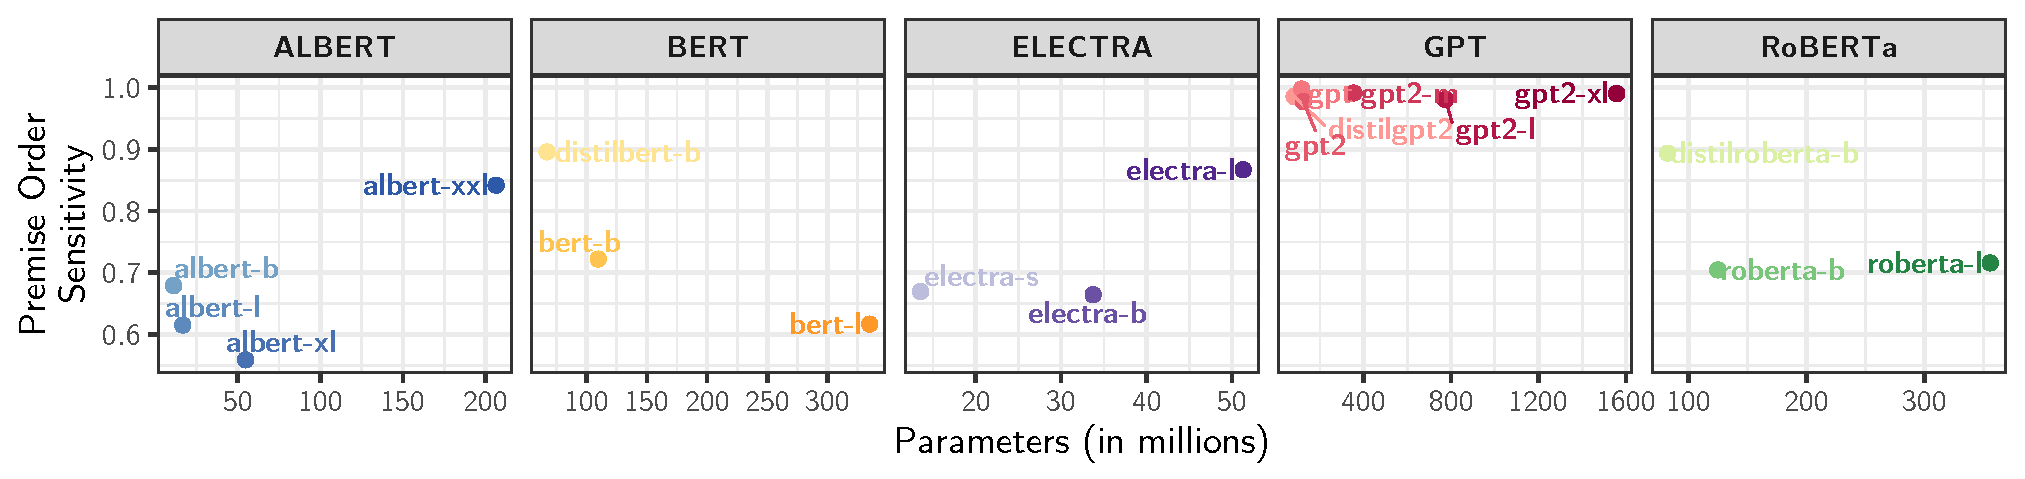
\includegraphics[width = \textwidth]{../paper/pos_confound.pdf}
    \caption{Model's sensitivity to changes in Premise word order.}
    \label{fig:cogsci21pos}
\end{figure}

\paragraph{Taxonomic Sensitivity}
LMs might tend to repeat the property phrase mentioned in the predicted material with high probability when prefixed by a sentence containing it, i.e., repeating \textit{``can dax''} in the conclusion when already conditioned on the same phrase in the premise \citep{holtzman2019curious}, confounding the degree to which the conclusion is generated using the taxonomic relationship between the premise and the conclusion categories.
In order to study this tendency, we compute the LMs' probabilities for conclusions consisting of a different category with the exact same property as the original (for instance, \textit{``All fruits are slithy''} given \textit{``Sofas are slithy''}). We call this measure $AS_{\textit{flipped}}$. Just like in our POS calculation, our TS measure for each item is calculated as the difference between the original measure and the flipped measure:
\begin{align}
    \text{TS}_i = AS_i - AS_{\textit{flipped}, i}
\end{align}
As is the case with POS, it is desirable to have a strongly positive value for sensitivity towards this confound (i.e., TS $>$ 0). 
\Cref{fig:cogsci21ts} shows the the proportion of cases (out of 12{,}180 for each model) where TS was greater than 0, against the models' total number of trainable parameters.
From \Cref{fig:cogsci21ts}, there is a non-trivial proportion of cases where models produce greater $AS$ scores for the conclusion when the premise concept had no taxonomic relation to the conclusion concept as compared to when it did, suggesting that in many cases models might not be processing based on the taxonomic relation between premise and conclusion and may simply be assigning high probabilities to the property phrase because it was listed in the preceding context -- it is common-knowledge that LMs are highly conducive to repeating text already seen in the input context \citep{holtzman2019curious}.

\begin{figure}[!th]
    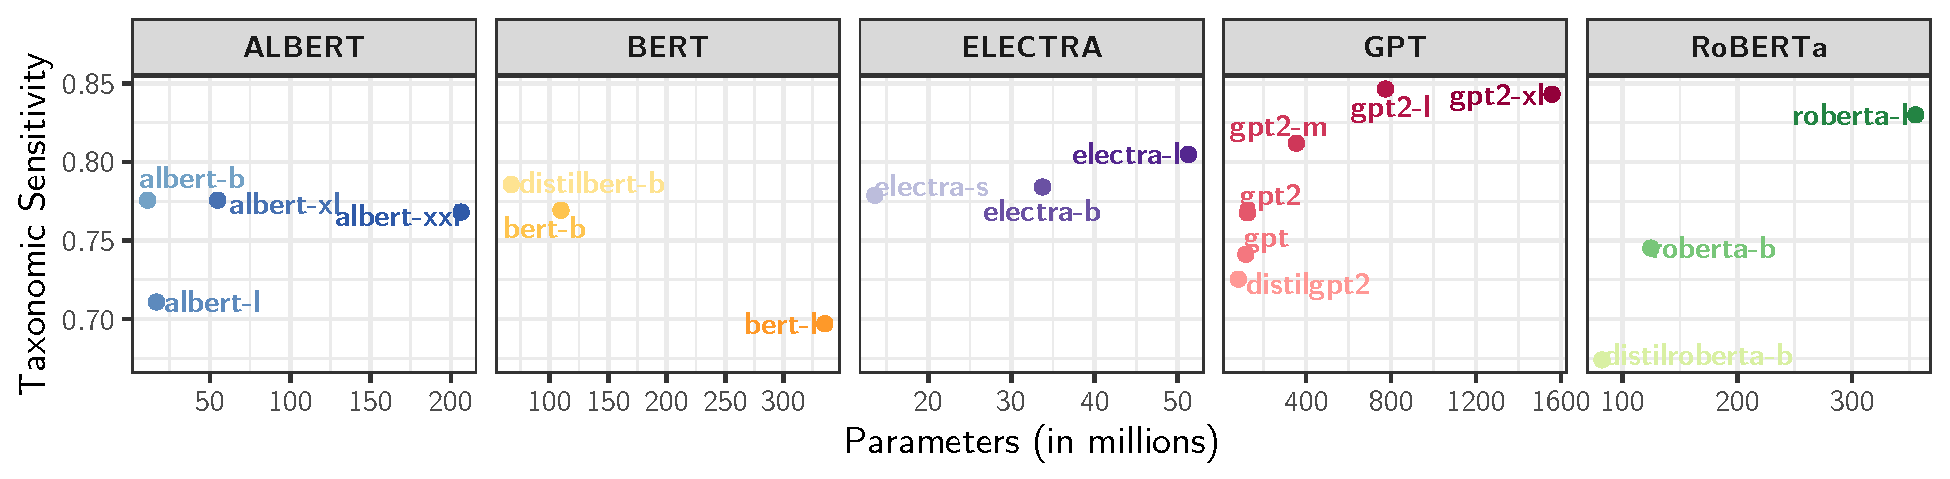
\includegraphics[width = \textwidth]{../paper/ts_confound.pdf}
    \caption{Models' sensitivities to violation of the taxonomic relation between the premise and the conclusion categories.}
    \label{fig:cogsci21ts}
\end{figure}

\section{Additional Results}
\subsection{Category-wise results on Taxonomic Sentence Verification Experiments}

See \Cref{fig:tsvcategory}.

\begin{figure}[h]
    \centering
    \begin{subfigure}[b]{\textwidth}
        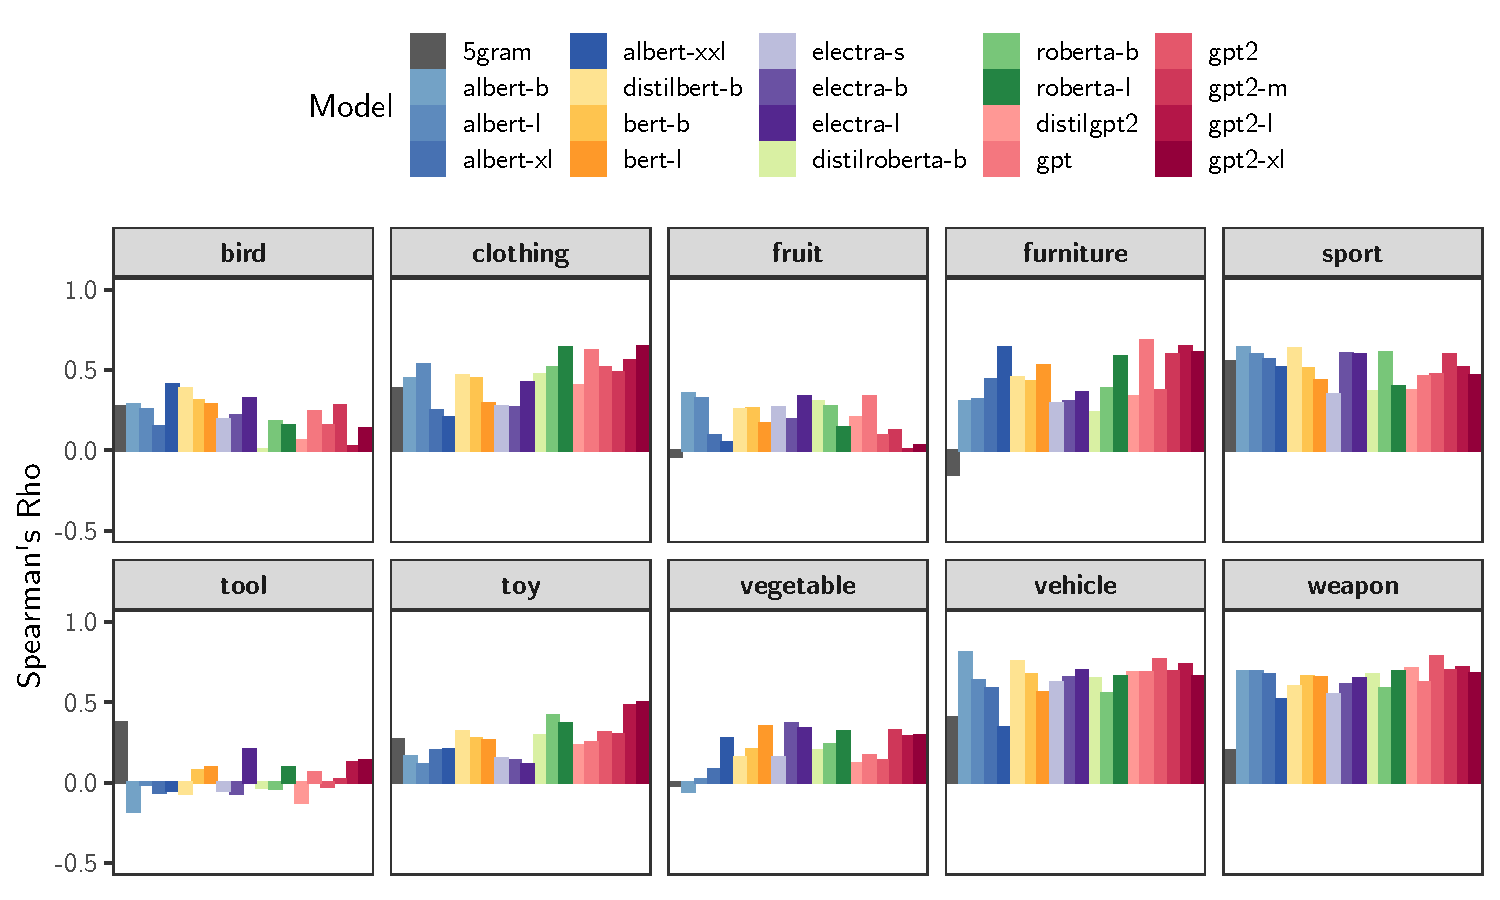
\includegraphics[width = \textwidth]{../paper/tsv_categorywise.pdf}
        \caption{}
    \end{subfigure}\\
    \vspace{1em}
    \begin{subfigure}[b]{\textwidth}
        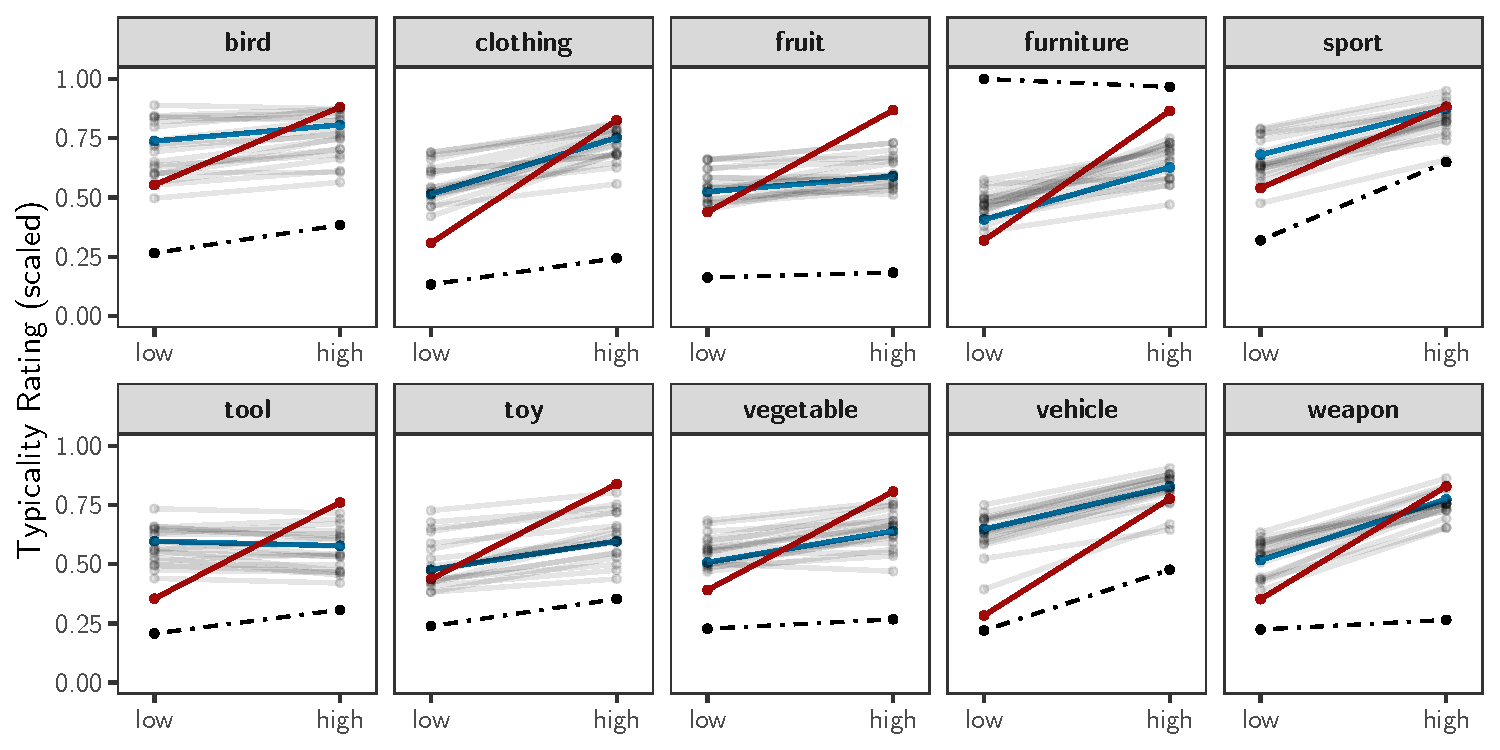
\includegraphics[width = \textwidth]{../paper/categorywisetsv.pdf}
        \caption{}
    \end{subfigure}
    \caption{Category-wise results from the \textbf{Taxonomic Sentence Verification} experiments -- (a) Spearman's correlation between language model log-probabilities and human typicality ratings; (b) Average scores (log-probability for language models, and raw typicality ratings for humans) assigned to low and high typicality items.}
    \label{fig:tsvcategory}
\end{figure}

\subsection{Category-wise results on Category-based Induction Experiments}

See \Cref{fig:cbicategory}.

\begin{figure}[h]
    \centering
    \begin{subfigure}[b]{\textwidth}
        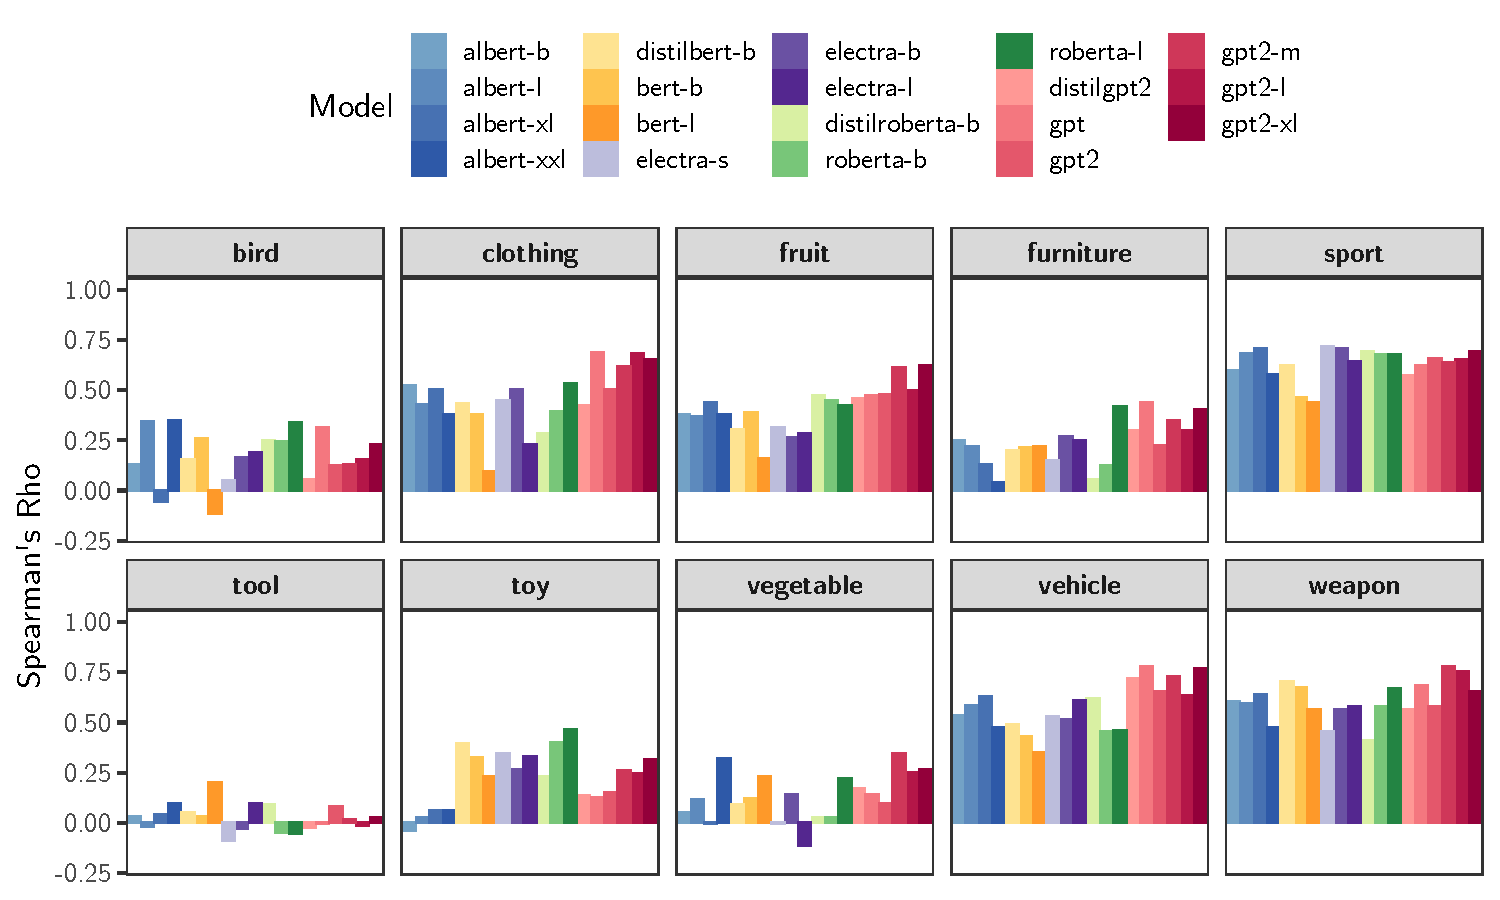
\includegraphics[width = \textwidth]{../paper/induction_categorywise.pdf}
        \caption{}
    \end{subfigure}\\
    \vspace{1em}
    \begin{subfigure}[b]{\textwidth}
        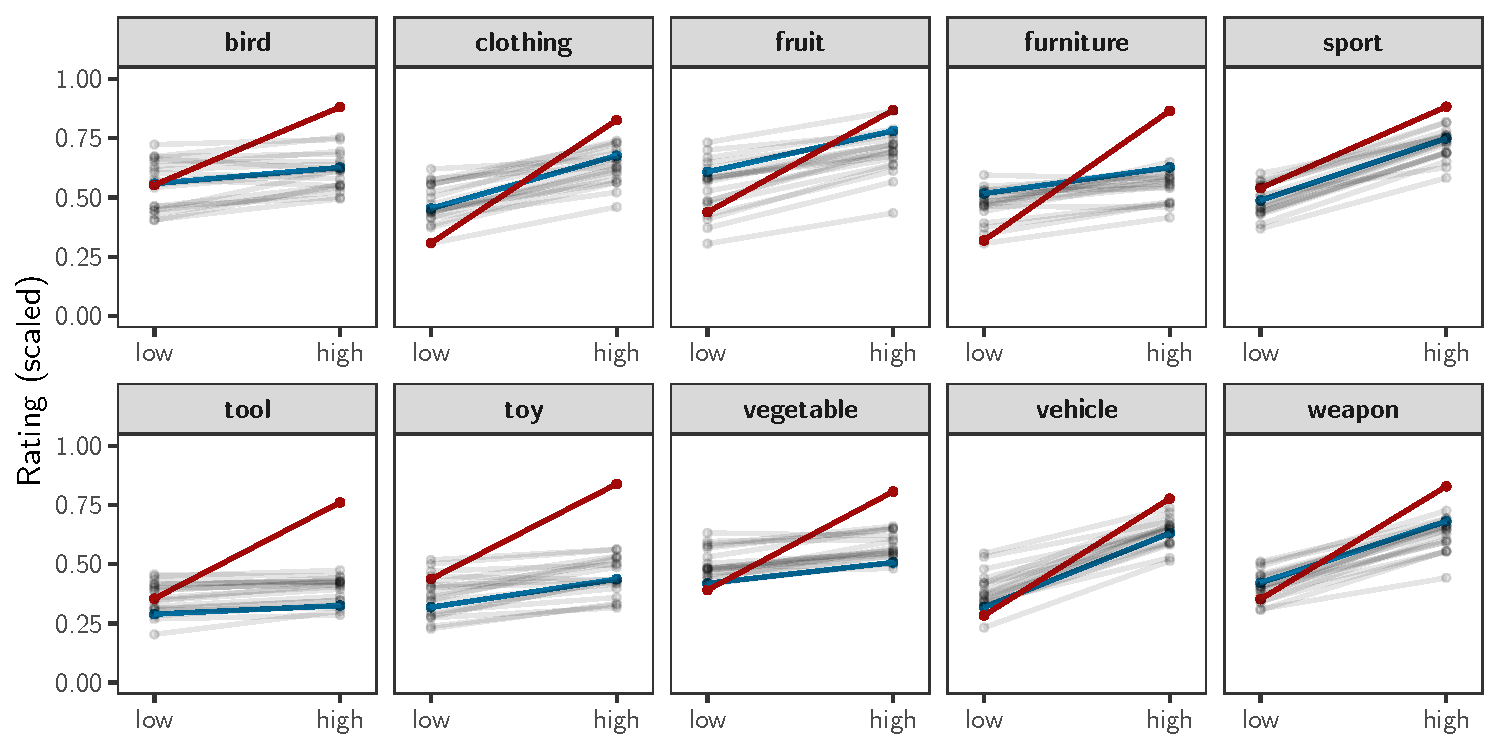
\includegraphics[width = \textwidth]{../paper/inductioncategorywiselowhigh.pdf}
        \caption{}
    \end{subfigure}
    \caption{Category-wise results from the \textbf{Category-based Induction} experiments -- (a) Spearman's correlation between adjusted $AS$-scores and human typicality ratings; (b) Average scores (adjusted $AS$-scores for language models, and raw typicality ratings for humans) assigned to low and high typicality items.}
    \label{fig:cbicategory}
\end{figure}


% \subsection{Typicality Correspondence and Model Parameters}

\bibliographystyle{acl}
\bibliography{references.bib}

\end{document}
